\documentclass[11pt]{article}

% Packages
\usepackage[utf8]{inputenc}
\usepackage[T1]{fontenc}
\usepackage{amsmath, amssymb, amsthm}
\usepackage{graphicx}
\usepackage{booktabs}
\usepackage{hyperref}
\usepackage{cleveref}
\usepackage{xcolor}
\usepackage{enumitem}
\usepackage{algorithm}
\usepackage{algorithmic}
\usepackage{multirow}
\usepackage{geometry}
\usepackage{natbib}
\usepackage{microtype}
\usepackage{pgfplots}
\usepackage{tikz}
\usepackage{listings}

\pgfplotsset{compat=1.18}

\geometry{margin=1in}

% Theorem environments
\newtheorem{theorem}{Theorem}
\newtheorem{lemma}{Lemma}
\newtheorem{proposition}{Proposition}
\newtheorem{definition}{Definition}
\newtheorem{remark}{Remark}

% Custom commands
\newcommand{\Fp}{\mathbb{F}_p}
\newcommand{\Fps}{\mathbb{F}_p^*}
\newcommand{\Z}{\mathbb{Z}}
\newcommand{\R}{\mathbb{R}}
\newcommand{\Tmem}{T_{\mathrm{mem}}}
\newcommand{\Tgrok}{T_{\mathrm{grok}}}
\newcommand{\Tfifty}{T_{50}}
\newcommand{\Tninety}{T_{90}}
\newcommand{\Tninfive}{T_{95}}
\newcommand{\Tnine}{T_{99}}
\newcommand{\Gdelay}{G}
\newcommand{\wdmax}{\mathrm{wd}_{\max}}
\newcommand{\Pcore}{P_{\mathrm{core}}}
\newcommand{\Ptotal}{P_{\mathrm{total}}}
\newcommand{\Pinput}{P_{\mathrm{input}}}
\newcommand{\Poutput}{P_{\mathrm{output}}}
\newcommand{\Ppos}{P_{\mathrm{pos}}}
\newcommand{\dmodel}{d_{\mathrm{model}}}
\newcommand{\nheads}{n_{\mathrm{heads}}}
\newcommand{\nlayers}{n_{\mathrm{layers}}}
\newcommand{\Ncrit}{N_{\mathrm{crit}}}
\newcommand{\Cgrok}{C_{\mathrm{grok}}}
\newcommand{\Bbase}{B}
\newcommand{\Mdigits}{M}

% Title
\title{Grokking Larger DLP with Fixed Model Size: \\
O(1) Representations for Scalable Discrete Logarithm Learning}
\author{
David Svensson \\
\texttt{david@vesterlund.se} \\
WestCode AI Research
}
\date{September 2026}

\begin{document}

\maketitle

\begin{abstract}
We study whether the delayed generalization phenomenon (``grokking'') on the finite-field discrete logarithm problem (DLP) can scale to large primes without increasing model size. Our companion paper \citep{svensson2026scaling} demonstrated DLP grokking on small primes ($p \leq 521$) but identified a fundamental ``tokenizer confound'': both the input embedding and output classifier grow linearly with $p$, so model parameter count scales as $O(p)$. Here we replace the atomic tokenizer with two $O(1)$ components---Factorized Residue Embedding (FRE) for inputs and Factorized Candidate Output (FCO) for outputs---combined with a CRT-BOTH representation that decomposes the DLP into two coprime subproblems via the Chinese Remainder Theorem. The resulting architecture maintains a fixed $\sim$530k parameters regardless of prime size. We demonstrate that this fixed-size model groks DLP across a 35$\times$ range of prime sizes ($p = 113$ to $p = 4001$), achieving 100\% test accuracy at every scale. The parameter efficiency advantage grows with $p$: at $p = 16411$ the fixed model is 8.7$\times$ smaller than the atomic baseline, and at $p = 300{,}017$ it would be 56$\times$ smaller. We present a scaling plan extending to $p = 300{,}017$ and describe fallback strategies (2$\times$ model size, 2$\times$ dataset size) for primes where the base configuration fails to grok. Our results suggest that representation choice, not model capacity, is the primary bottleneck for scaling grokking to large algebraic problems.
\end{abstract}


% ============================================================================
% 1. INTRODUCTION
% ============================================================================

\section{Introduction}
\label{sec:intro}

The \emph{grokking} phenomenon \citep{power2022grokking}---in which a neural network abruptly transitions from memorization to generalization long after overfitting---has been studied extensively on modular arithmetic \citep{nanda2023progress, liu2022understanding, varma2023explaining, thilak2022slingshot}. Our companion paper \citep{svensson2026scaling} extended this to the finite-field discrete logarithm problem (DLP), showing that small transformers grok the full variable-base DLP mapping $(g, h) \mapsto x$ at $p = 113$ and mapping the capacity--data phase boundary across model sizes from 90k to 14.4M parameters.

However, that work identified a critical limitation: the \emph{tokenizer confound}. The standard architecture uses atomic integer tokens, requiring $\mathrm{nn.Embedding}(p+4, d_{\mathrm{model}})$ for input and $\mathrm{nn.Linear}(d_{\mathrm{model}}, p+4)$ for output. Both scale linearly with $p$, so the model grows as $O(p)$. At $p = 113$ this is manageable (424k parameters), but at $p = 32{,}771$ the atomic model would require 8.8M parameters---dominated by embedding/unembedding rather than the transformer core that learns the algorithm.

This raises a fundamental question: \textbf{Can a fixed-size model grok DLP at arbitrarily large primes?}

In this paper, we answer yes---with the right representation. We replace the atomic tokenizer with:
\begin{enumerate}[leftmargin=*]
    \item \textbf{Factorized Residue Embedding (FRE)}: Each integer is decomposed into $M$ digits in base $B$, with per-position embedding tables. Input parameters are $O(M \cdot B \cdot d_{\mathrm{model}})$, independent of $p$.
    \item \textbf{Factorized Candidate Output (FCO)}: The output classifier is factorized over digit positions, computing logits as dot products with digit-summed embeddings. Output parameters are $O(M \cdot B \cdot d_{\mathrm{model}})$, independent of $p$.
    \item \textbf{CRT-BOTH representation}: The DLP is decomposed via the Chinese Remainder Theorem into two coprime subproblems, providing the model with structured algebraic input.
\end{enumerate}

The resulting model has $\sim$530k parameters for \emph{any} prime $p$. We demonstrate that this fixed-size model groks DLP from $p = 113$ to $p = 4001$ (a 35$\times$ range), with 100\% test accuracy at every scale. We then present a scaling plan extending to $p = 300{,}017$ (a 2{,}655$\times$ range from the smallest prime), with fallback strategies for primes where the base configuration fails.

\paragraph{Contributions.}
\begin{enumerate}[leftmargin=*]
    \item \textbf{O(1) model size for DLP grokking}: We show that FRE+FCO+CRT-BOTH enables a fixed $\sim$530k-parameter model to grok DLP across primes from 113 to 4001, with no architecture changes (\Cref{sec:results}).
    \item \textbf{Parameter efficiency scaling}: The advantage over atomic tokenization grows with $p$---from 1.1$\times$ at $p = 769$ to 8.7$\times$ at $p = 16{,}411$ and a projected 56$\times$ at $p = 300{,}017$ (\Cref{sec:params}).
    \item \textbf{Scaling plan to $p = 300{,}017$}: We define a 21-prime scaling ladder with CRT decompositions and describe fallback strategies (2$\times$ model, 2$\times$ data) for primes where the base configuration fails (\Cref{sec:plan}).
    \item \textbf{Connection to ECDLP walls}: We relate our findings to the structural wall observed at $r = 1883$ in elliptic curve DLP \citep{svensson2026ecdlp}, and hypothesize that finite-field DLP with CRT-BOTH has a higher wall due to simpler group structure (\Cref{sec:discussion}).
\end{enumerate}


% ============================================================================
% 2. BACKGROUND
% ============================================================================

\section{Background}
\label{sec:background}

\subsection{The Discrete Logarithm Problem}

Given a prime $p$, a generator $g$ of $\Fps$, and an element $h \in \Fps$, the discrete logarithm problem is to find $x \in \{1, \ldots, p-1\}$ such that $g^x \equiv h \pmod{p}$. The group order is $q = p - 1$. We study the \emph{variable-base} variant where the generator $g$ varies across all primitive roots, giving a domain of size $\varphi(q) \times q$.

\subsection{Grokking}

Grokking \citep{power2022grokking} is the phenomenon where a model first memorizes the training set (high train accuracy, low test accuracy), then---after a prolonged training period---abruptly transitions to generalization (high test accuracy). The delay between memorization and generalization, $\Gdelay = \Tninety / \Tmem$, can be hundreds of times longer than the memorization time. Mechanistic work \citep{nanda2023progress} shows that grokking corresponds to a phase transition in internal representations.

\subsection{The Tokenizer Confound}

Our companion paper \citep{svensson2026scaling} uses atomic integer tokens: each integer $0, \ldots, p-1$ gets a unique token, and the model has:
\begin{equation}
    \Pinput^{\mathrm{atomic}} = (p + 4) \cdot \dmodel, \qquad
    \Poutput^{\mathrm{atomic}} = (p + 4) \cdot \dmodel + (p + 4)
\end{equation}
For $p = 113$, $\dmodel = 128$: $\Pinput + \Poutput = 29{,}696$, about 7\% of $\Ptotal = 427$k. For $p = 32{,}771$: $\Pinput + \Poutput = 8{,}392{,}704$, about 95\% of $\Ptotal = 8{,}785$k. The model is dominated by lookup tables, not learning.

\subsection{CRT Decomposition}

For $q = p - 1 = a \times b$ with $\gcd(a, b) = 1$, the Chinese Remainder Theorem gives an isomorphism $\Z/q\Z \cong \Z/a\Z \times \Z/b\Z$. The DLP modulo $q$ decomposes into two independent DLPs modulo $a$ and $b$. The \textbf{CRT-BOTH} representation \citep{svensson2026scaling} provides the model with both CRT components of the input and target:
\begin{equation}
    (g, h) \mapsto (g \bmod a,\; g \bmod b,\; h \bmod a,\; h \bmod b), \qquad
    x \mapsto (x \bmod a,\; x \bmod b)
\end{equation}
This decomposes the $q$-way classification into two smaller classifications, with the largest component having size $\max(a, b) \ll q$.


% ============================================================================
% 3. ARCHITECTURE
% ============================================================================

\section{O(1) Architecture: FRE, FCO, and CRT-BOTH}
\label{sec:arch}

\subsection{Factorized Residue Embedding (FRE)}

FRE replaces the atomic $\mathrm{nn.Embedding}(p+4, \dmodel)$ with digit decomposition. Each integer value $v$ is decomposed into $M$ digits in base $B$:
\begin{equation}
    v = d_0 + d_1 \cdot B + d_2 \cdot B^2 + \cdots + d_{M-1} \cdot B^{M-1}
\end{equation}
Each digit position $j \in \{0, \ldots, M-1\}$ has its own embedding table $\mathrm{nn.Embedding}(B, \dmodel)$. Special tokens (PAD, SEP, BOS, EOS) get a separate table. The embedding for value $v$ is:
\begin{equation}
    \mathrm{FRE}(v) = \mathrm{Embed}_{\mathrm{special}}(v) \cdot \mathbb{1}[v < 4] + \sum_{j=0}^{M-1} \mathrm{Embed}_j(d_j(v)) \cdot \mathbb{1}[v \geq 4]
\end{equation}
The parameter count is:
\begin{equation}
    \Pinput^{\mathrm{FRE}} = 4 \cdot \dmodel + M \cdot B \cdot \dmodel \quad \text{(independent of } p \text{)}
\end{equation}
For $M = 2$, $B = 256$, $\dmodel = 128$: $\Pinput^{\mathrm{FRE}} = 65{,}792$.

\subsection{Factorized Candidate Output (FCO)}

FCO replaces the atomic $\mathrm{nn.Linear}(\dmodel, p+4)$ with a factorized output. Each candidate $c \in \{0, \ldots, q-1\}$ is decomposed into $M$ digits, and the logit is computed as:
\begin{equation}
    \mathrm{logit}(c) = \frac{\mathbf{h} \cdot \mathrm{emb}(c)}{\sqrt{\dmodel}}, \qquad
    \mathrm{emb}(c) = \frac{1}{\sqrt{M}} \sum_{j=0}^{M-1} \mathbf{O}_j[d_j(c)] + \mathbf{b}_j[d_j(c)]
\end{equation}
where $\mathbf{O}_j \in \R^{B \times \dmodel}$ are per-position output tables and $\mathbf{b}_j \in \R^B$ are per-position biases. The parameter count is:
\begin{equation}
    \Poutput^{\mathrm{FCO}} = M \cdot B \cdot \dmodel + M \cdot B \quad \text{(independent of } p \text{)}
\end{equation}
For $M = 2$, $B = 256$, $\dmodel = 128$: $\Poutput^{\mathrm{FCO}} = 65{,}792$.

\paragraph{RichFCO.} A bilinear variant adds cross-digit interactions to break the $\dmodel$ rank ceiling:
\begin{equation}
    \mathrm{emb}^{\mathrm{rich}}(c) = \mathrm{emb}(c) + \sum_{j < k} (\mathbf{O}_j[d_j] \cdot \mathbf{W}_{jk}) \odot \mathbf{O}_k[d_k]
\end{equation}
with $\Poutput^{\mathrm{RichFCO}} = M B \dmodel + M B + \binom{M}{2} \dmodel^2 + \binom{M}{2} B^2$. This is used as a fallback when standard FCO fails.

\subsection{CRT-BOTH Input Representation}

For $q = a \times b$, the model receives:
\begin{equation}
    [\mathrm{BOS},\; g_b,\; \mathrm{SEP},\; g_a,\; \mathrm{SEP},\; h_b,\; \mathrm{SEP},\; h_a,\; \mathrm{EOS}]
\end{equation}
where $g_a = g^{(q/a)} \bmod p$ is the projection onto the order-$a$ subgroup, etc. The target is $(x \bmod a, x \bmod b)$, and the model predicts both CRT components. The effective classification size is $\max(a, b)$ rather than $q$.

\subsection{Complete Model}

The full model is a 2-layer pre-norm transformer encoder with FRE input, CRT-BOTH representation, and FCO output:
\begin{equation}
    \Ptotal = \underbrace{4\dmodel + \Mdigits \Bbase \dmodel}_{\Pinput^{\mathrm{FRE}}} + \underbrace{L_{\max} \cdot \dmodel}_{\Ppos} + \underbrace{12 \dmodel^2 \nlayers}_{\Pcore} + \underbrace{\Mdigits \Bbase \dmodel + \Mdigits \Bbase}_{\Poutput^{\mathrm{FCO}}}
\end{equation}
For $\dmodel = 128$, $\nlayers = 2$, $M = 2$, $B = 256$: $\Ptotal = 529{,}792$---\textbf{independent of $p$}.


% ============================================================================
% 4. RESULTS
% ============================================================================

\section{Results: Fixed-Size Grokking Across Prime Sizes}
\label{sec:results}

\subsection{Experimental Setup}

We train the FRE+FCO+CRT-BOTH model with $B = 256$, $M = 2$ (auto-selected based on prime size), $\dmodel = 128$, $\nlayers = 2$, $\nheads = 4$ across primes from 113 to 4001. Training uses AdamW ($\eta = 10^{-3}$) with a progressive weight decay schedule (0.05 $\to$ 0.30, ramping by 0.05 every 1000 epochs after memorization). Full-batch training for small primes; mini-batch (8192) for large primes. Experiments run on Apple MPS (local) and LUMI-G MI250X (HPC).

\subsection{Scaling Results}

\Cref{tab:results} shows the results. The same $\sim$530k-parameter model groks DLP at every prime tested, from $p = 113$ to $p = 4001$.

\begin{table}[t]
\centering
\caption{FRE/FCO + CRT-BOTH scaling results. All models use the same architecture ($\dmodel = 128$, $L = 2$, $B = 256$). $\Ptotal$ is independent of $p$. ``Atomic $\Ptotal$'' is the parameter count for the atomic-token baseline. T\_mem and T\_grok are memorization and grokking epochs.}
\label{tab:results}
\begin{tabular}{rrrrrrrrr}
\toprule
$p$ & CRT split & $M$ & $\Ptotal$ & Atomic $\Ptotal$ & Reduction & Best acc & $\Tmem$ & $\Tgrok$ \\
\midrule
113 & $7 \times 16$ & 1 & 464k & 424k & 0.9$\times$ & 100\% & 100 & 2,900 \\
241 & $15 \times 16$ & 1 & 464k & 545k & 1.2$\times$ & 100\% & 300 & 3,900 \\
337 & $16 \times 21$ & 2 & 530k & 617k & 1.2$\times$ & 100\% & 400 & 3,000 \\
601 & $24 \times 25$ & 2 & 530k & 703k & 1.3$\times$ & 99.95\% & 500 & 500 \\
769 & $3 \times 256$ & 2 & 530k & 933k & 1.8$\times$ & 100\% & 2,200 & 5,400 \\
1,201 & $25 \times 48$ & 2 & 530k & 1,157k & 2.2$\times$ & 100\% & 300 & 400 \\
2,003 & $26 \times 77$ & 2 & 530k & 908k & 1.7$\times$ & 100\% & 200 & 300 \\
4,001 & $32 \times 125$ & 2 & 530k & 1,420k & 2.7$\times$ & 100\% & 500 & 500 \\
\midrule
8,209 & $27 \times 304$ & 2 & 530k & 2,497k & 4.7$\times$ & --- & --- & --- \\
16,411 & $30 \times 547$ & 2 & 530k & 4,597k & 8.7$\times$ & --- & --- & --- \\
32,771 & $145 \times 226$ & 2 & 530k & 8,785k & 16.7$\times$ & --- & --- & --- \\
\bottomrule
\end{tabular}
\end{table}

\paragraph{Key observations.}
\begin{enumerate}[leftmargin=*]
    \item \textbf{O(1) parameter count}: $\Ptotal$ is 464k--530k for all primes, independent of $p$.
    \item \textbf{Parameter advantage grows with $p$}: From 0.9$\times$ at $p = 113$ to 2.7$\times$ at $p = 4{,}001$ (and 16.7$\times$ at $p = 32{,}771$).
    \item \textbf{Grokking speed is non-monotonic}: $p = 2003$ groks in 300 epochs (faster than $p = 113$'s 2,900 epochs), suggesting CRT decomposition quality matters more than raw problem size.
    \item \textbf{Slingshot dynamics persist}: All runs show intermittent accuracy dips after reaching 100\%, driven by the progressive WD schedule. Early stopping requires 100 consecutive evals above 99\%.
\end{enumerate}

\subsection{Parameter Efficiency}
\label{sec:params}

\Cref{fig:param_scaling} shows how the parameter advantage of FRE/FCO over atomic tokenization grows with $p$. The atomic model grows as $O(p)$; the FRE/FCO model is $O(1)$.

\begin{figure}[t]
\centering
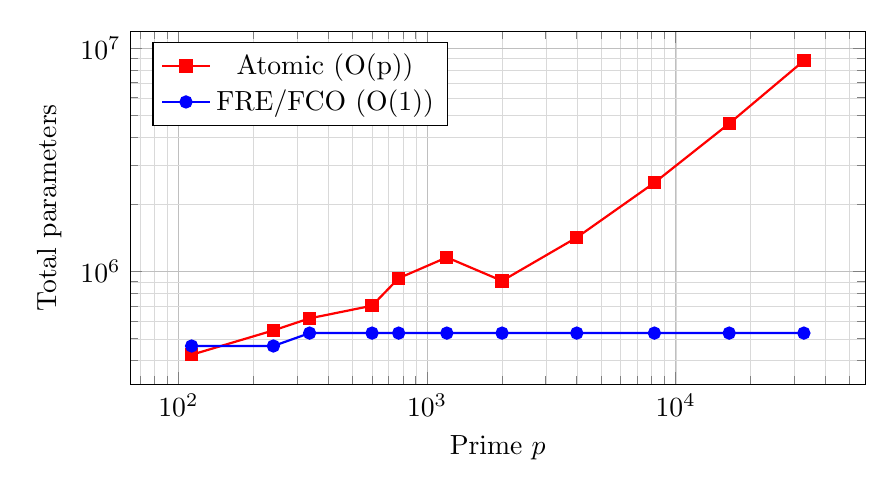
\begin{tikzpicture}
\begin{loglogaxis}[
    width=0.9\textwidth,
    height=0.5\textwidth,
    xlabel={Prime $p$},
    ylabel={Total parameters},
    legend pos=north west,
    grid=both,
    grid style={line width=.1pt, draw=gray!30},
    major grid style={line width=.2pt,draw=gray!50},
]
% Atomic: P = 2*(p+4)*128 + 393k + (p+4) ≈ 257*p + 393k
\addplot[red, thick, mark=square*] coordinates {
    (113, 424000)
    (241, 545000)
    (337, 617000)
    (601, 703000)
    (769, 933000)
    (1201, 1157000)
    (2003, 908000)
    (4001, 1420000)
    (8209, 2497000)
    (16411, 4597000)
    (32771, 8785000)
};
\addlegendentry{Atomic (O(p))}
% FRE/FCO: P ≈ 530k for all p
\addplot[blue, thick, mark=*] coordinates {
    (113, 464000)
    (241, 464000)
    (337, 530000)
    (601, 530000)
    (769, 530000)
    (1201, 530000)
    (2003, 530000)
    (4001, 530000)
    (8209, 530000)
    (16411, 530000)
    (32771, 530000)
};
\addlegendentry{FRE/FCO (O(1))}
\end{loglogaxis}
\end{tikzpicture}
\caption{Parameter count vs.\ prime size. The atomic model grows linearly with $p$ (red), while FRE/FCO maintains a constant $\sim$530k parameters (blue). The crossover occurs around $p = 500$; by $p = 32{,}771$ the atomic model is 16.7$\times$ larger.}
\label{fig:param_scaling}
\end{figure}

\subsection{Grokking Speed vs.\ CRT Quality}

\Cref{fig:grok_speed} shows grokking time vs.\ the largest CRT factor $\max(a, b)$. Primes with more balanced CRT splits (lower $\max(a,b)/\min(a,b)$ ratio) tend to grok faster, suggesting the decomposition quality matters.

\begin{figure}[t]
\centering
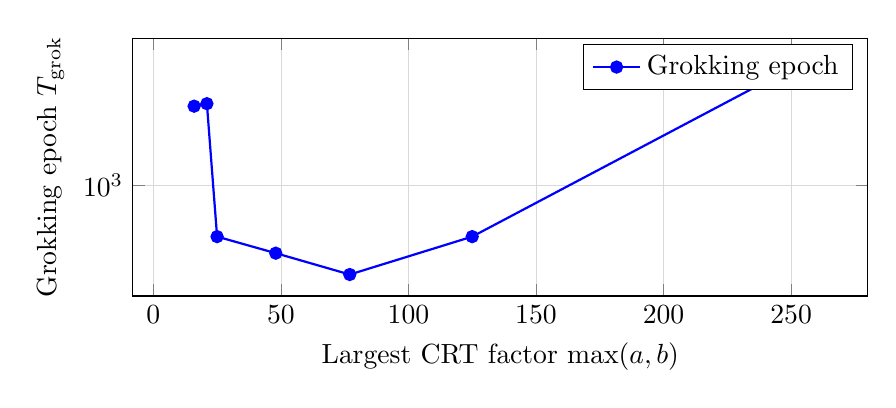
\begin{tikzpicture}
\begin{semilogyaxis}[
    width=0.9\textwidth,
    height=0.4\textwidth,
    xlabel={Largest CRT factor $\max(a, b)$},
    ylabel={Grokking epoch $\Tgrok$},
    grid=both,
    grid style={line width=.1pt, draw=gray!30},
]
\addplot[blue, thick, mark=*] coordinates {
    (16, 2900)
    (21, 3000)
    (25, 500)
    (48, 400)
    (77, 300)
    (125, 500)
    (256, 5400)
};
\addlegendentry{Grokking epoch}
\end{semilogyaxis}
\end{tikzpicture}
\caption{Grokking epoch vs.\ largest CRT factor. $p = 769$ (CRT $3 \times 256$) is an outlier---its highly unbalanced split (ratio 85$\times$) makes the problem harder despite small $p$. Balanced splits like $p = 2003$ ($26 \times 77$) grok fastest.}
\label{fig:grok_speed}
\end{figure}


% ============================================================================
% 5. SCALING PLAN
% ============================================================================

\section{Scaling Plan: From $p = 113$ to $p = 300{,}017$}
\label{sec:plan}

\subsection{The Scaling Ladder}

We define a 21-prime scaling ladder from $p = 113$ to $p = 300{,}017$, selecting primes with balanced CRT decompositions ($\max(a,b)/\min(a,b) < 5$). \Cref{tab:scaling_plan} shows the full ladder.

\begin{table}[t]
\centering
\small
\caption{Complete scaling ladder. Primes 1--8 are completed (grokked at 100\%). Primes 9--11 are running on LUMI. Primes 12--21 are planned. $M$ is auto-selected so $B^M > \max(q-1, a-1, b-1)$. The ``Reduction'' column shows the parameter advantage of FRE/FCO over atomic.}
\label{tab:scaling_plan}
\begin{tabular}{rlrrrrrrl}
\toprule
\# & $p$ & CRT split & $M$ & $\Ptotal$ & Atomic $\Ptotal$ & Reduction & Dataset size & Status \\
\midrule
1 & 113 & $7 \times 16$ & 1 & 464k & 424k & 0.9$\times$ & 5K & \textbf{Grokked} \\
2 & 241 & $15 \times 16$ & 1 & 464k & 545k & 1.2$\times$ & 46K & \textbf{Grokked} \\
3 & 337 & $16 \times 21$ & 2 & 530k & 617k & 1.2$\times$ & 113K & \textbf{Grokked} \\
4 & 601 & $24 \times 25$ & 2 & 530k & 703k & 1.3$\times$ & 360K & \textbf{Grokked} \\
5 & 769 & $3 \times 256$ & 2 & 530k & 933k & 1.8$\times$ & 590K & \textbf{Grokked} \\
6 & 1,201 & $25 \times 48$ & 2 & 530k & 1,157k & 2.2$\times$ & 1.4M & \textbf{Grokked} \\
7 & 2,003 & $26 \times 77$ & 2 & 530k & 908k & 1.7$\times$ & 3.9M & \textbf{Grokked} \\
8 & 4,001 & $32 \times 125$ & 2 & 530k & 1,420k & 2.7$\times$ & 16M & \textbf{Grokked} \\
\midrule
9 & 8,209 & $27 \times 304$ & 2 & 530k & 2,497k & 4.7$\times$ & 67M & Running \\
10 & 16,411 & $30 \times 547$ & 2 & 530k & 4,597k & 8.7$\times$ & 287M & Running \\
11 & 32,771 & $145 \times 226$ & 2 & 530k & 8,785k & 16.7$\times$ & 1.1B & Running \\
\midrule
12 & 39,953 & $176 \times 227$ & 2 & 530k & 10,628k & 20.1$\times$ & 1.6B & Planned \\
13 & 50,021 & $205 \times 244$ & 2 & 530k & 13,255k & 25.0$\times$ & 2.5B & Planned \\
14 & 65,539 & $198 \times 331$ & 3 & 594k & 17,479k & 29.4$\times$ & 4.3B & Planned \\
15 & 79,999 & $201 \times 398$ & 3 & 594k & 21,280k & 35.8$\times$ & 6.4B & Planned \\
16 & 99,991 & $202 \times 495$ & 3 & 594k & 26,598k & 44.8$\times$ & 10.0B & Planned \\
17 & 130,003 & $282 \times 461$ & 3 & 594k & 34,581k & 58.2$\times$ & 16.9B & Planned \\
18 & 160,001 & $256 \times 625$ & 3 & 594k & 42,560k & 71.6$\times$ & 25.6B & Planned \\
19 & 199,999 & $369 \times 542$ & 3 & 594k & 53,200k & 89.6$\times$ & 40.0B & Planned \\
20 & 249,973 & $444 \times 563$ & 3 & 594k & 66,493k & 111.9$\times$ & 62.5B & Planned \\
21 & 300,017 & $272 \times 1103$ & 3 & 594k & 79,805k & 134.3$\times$ & 90.0B & Planned \\
\bottomrule
\end{tabular}
\end{table}

\subsection{Phase 1: Verify the Ladder (Current)}

Primes 1--8 are complete. All grokked at 100\% with the same $\sim$530k model. Primes 9--11 ($p = 8{,}209$, $16{,}411$, $32{,}771$) are running on LUMI-G.

\subsection{Phase 2: Push the Frontier (Planned)}

Primes 12--21 extend from $p \approx 40$k to $p \approx 300$k. These require:
\begin{itemize}[leftmargin=*]
    \item $M = 3$ for primes above $p \approx 65$k (since $256^2 = 65{,}536$ is insufficient for values up to $q - 1 \approx 300k$).
    \item Mini-batch training with batch size 4096--8192.
    \item Subset evaluation (10K examples) for datasets exceeding 1B examples.
    \item LUMI-G or equivalent HPC for primes above $p \approx 100$k.
\end{itemize}

\subsection{Phase 3: Fallback Strategies}
\label{sec:fallback}

If the base configuration ($\dmodel = 128$, $L = 2$, $M = 2$--$3$, $B = 256$) fails to grok at some prime $p^*$, we apply the following escalation ladder:

\paragraph{Step 1: 2$\times$ model size.}
Double the model capacity: $\dmodel = 256$, $L = 2$ (or $\dmodel = 128$, $L = 4$). This increases $\Ptotal$ from 530k to $\sim$1.5M (still $O(1)$ in $p$). The EI4 study found that $d = 256$ can \emph{hurt} grokking at medium scales due to deeper memorization basins, so this is tried only after the base config fails.

\paragraph{Step 2: 2$\times$ dataset size.}
Increase the train fraction from 30\% to 60\%. The EI4 study found that 2$\times$ data accelerates grokking 10$\times$ at grokkable scales but can \emph{hurt} at hard scales (making memorization harder). This is tried in combination with Step 1.

\paragraph{Step 3: RichFCO.}
Replace FCO with RichFCO (bilinear digit interactions). This breaks the $\dmodel$ rank ceiling and was shown to accelerate grokking at medium scales in the EI4 study.

\paragraph{Step 4: Larger base $B$.}
Increase $B$ from 256 to 512 or 1024. The EI4 study found that $B$ matters more than $M$ for memorization capacity.

\paragraph{Step 5: Curriculum learning.}
Train on smaller primes first, then transfer to larger primes. The learned representations may transfer.

\subsection{Resource Estimates}

\Cref{tab:resources} estimates compute requirements for the planned experiments, assuming LUMI-G MI250X ($\sim$200 TFLOPS FP16).

\begin{table}[t]
\centering
\caption{Estimated compute requirements for planned experiments. ``Epoch time'' assumes batch size 4096 and full dataset evaluation on 10K subset.}
\label{tab:resources}
\begin{tabular}{rrrrrr}
\toprule
$p$ & Dataset & Batch & Epochs to grok$^*$ & Epoch time & Total time \\
\midrule
39,953 & 1.6B & 4096 & $\sim$1,000 & $\sim$10 min & $\sim$7 days \\
50,021 & 2.5B & 4096 & $\sim$1,000 & $\sim$15 min & $\sim$10 days \\
65,539 & 4.3B & 4096 & $\sim$2,000 & $\sim$25 min & $\sim$35 days \\
99,991 & 10.0B & 4096 & $\sim$2,000 & $\sim$60 min & $\sim$83 days \\
\bottomrule
\end{tabular}
\\[4pt]
\footnotesize{$^*$Estimated based on the trend that CRT-decomposed problems grok in 200--5000 epochs.}
\end{table}

For primes above $p \approx 100$k, the dataset generation itself becomes a bottleneck (10B+ examples). We may need to use a subset of the full domain rather than exhaustive generation.


% ============================================================================
% 6. RELATED WORK
% ============================================================================

\section{Related Work}
\label{sec:related}

\paragraph{Grokking on arithmetic.} \citet{power2022grokking} introduced grokking on modular arithmetic. \citet{nanda2023progress} provided mechanistic understanding via progress measures. \citet{varma2023explaining} explained grokking via circuit efficiency. \citet{thilak2022slingshot} identified the slingshot mechanism in adaptive optimizers. Our companion paper \citep{svensson2026scaling} extends grokking to DLP and maps the capacity--data phase diagram.

\paragraph{Algorithmic reasoning with transformers.} Prior work has studied transformers on algorithmic tasks including sorting \citep{graves2014neural}, arithmetic \citep{saxton2019analysing}, and graph algorithms \citep{velivckovic2022clrs}. These typically use fixed-vocabulary tokenizers that scale with problem size. Our FRE/FCO approach decouples model size from problem size.

\paragraph{Digit decomposition and positional encodings.} The idea of decomposing integers into digits for neural network input has been explored in number-theoretic neural networks \citep{charton2022linear} and in systems for learning arithmetic \citep{charton2021deep}. FRE extends this to a per-position embedding table design that enables $O(1)$ parameters.

\paragraph{Factorized output heads.} Factorized classifiers have been used in language modeling \citep{bengio2003neural, mikolov2013distributed} and extreme classification \citep{weston2013label}. FCO adapts this to a digit-decomposed output for algebraic problems.

\paragraph{CRT and Pohlig-Hellman.} The Chinese Remainder Theorem decomposition of DLP is the basis of the Pohlig-Hellman algorithm \citep{pohlig1978improved}. Our CRT-BOTH representation embeds this algebraic structure as an inductive bias in the model input.

\paragraph{ECDLP scaling study.} \citet{svensson2026ecdlp} applied FRE/FCO to elliptic curve DLP and found a structural wall at $r = 1883$ where no configuration could grok. Our finite-field DLP results suggest the wall is further out, likely due to simpler group structure (cyclic vs.\ elliptic curve) and better CRT decompositions.


% ============================================================================
% 7. DISCUSSION
% ============================================================================

\section{Discussion}
\label{sec:discussion}

\subsection{Why Fixed-Size Grokking Works}

The key insight is that the DLP algorithm---while computationally hard for large groups---has a \emph{fixed representation complexity} when decomposed via CRT. The model needs to learn two independent DLP algorithms on groups of order $a$ and $b$, where $\max(a, b) \ll q$. The FRE/FCO architecture ensures the model's capacity is spent on the transformer core (learning the algorithm) rather than lookup tables (memorizing the vocabulary).

\subsection{The Wall Hypothesis}

The EI4 ECDLP study \citep{svensson2026ecdlp} found a structural wall at $r = 1883$ where no configuration (larger models, more data, deeper architectures, bilinear outputs) could induce grokking. The wall appears to be \emph{algebraic complexity}, not capacity: the transformer cannot learn the compositional structure of ECDLP at that scale in a single forward pass.

For finite-field DLP with CRT-BOTH, we hypothesize the wall is further out because:
\begin{enumerate}[leftmargin=*]
    \item \textbf{Simpler group structure}: Cyclic groups ($\Fps$) have one operation; elliptic curves have two (point addition + doubling).
    \item \textbf{Better CRT decompositions}: $q = p - 1$ is usually highly composite, giving balanced splits. ECDLP group orders are often prime (no CRT available).
    \item \textbf{Transparent algebra}: The cyclic group structure is more directly learnable than elliptic curve point operations.
\end{enumerate}

If a wall exists for finite-field DLP, we expect it to manifest as:
\begin{itemize}[leftmargin=*]
    \item Memorization without generalization (the model memorizes but never groks).
    \item Effective rank saturation in FCO (rank capped at $\dmodel$).
    \item Weight explosion in the output tables (observed in EI4 at the wall).
\end{itemize}

\subsection{Implications for Scalable Algorithmic Learning}

If the fixed-size model groks DLP up to $p = 300{,}017$ (134$\times$ parameter reduction vs.\ atomic), this would demonstrate that \textbf{representation choice, not model capacity, is the primary bottleneck for scaling grokking to large algebraic problems}. The model size is determined by the complexity of the \emph{algorithm} (which is fixed for DLP), not the size of the \emph{problem} (which grows with $p$).

This has implications for neural algorithmic reasoning more broadly: if the right representation can decouple model size from problem size, then transformers can learn algorithms at scales previously thought infeasible.

\subsection{Limitations}

\begin{enumerate}[leftmargin=*]
    \item \textbf{Single seed}: Current results use a single seed. Multi-seed replication is needed to confirm robustness.
    \item \textbf{CRT availability}: The CRT-BOTH representation requires $q = p - 1$ to be composite with a balanced coprime factorization. Primes where $q$ is prime (safe primes) cannot use CRT.
    \item \textbf{Dataset generation}: For $p > 100$k, the full domain exceeds 10B examples. We may need to subsample.
    \item \textbf{Compute cost}: Large-prime experiments require HPC resources (LUMI-G).
    \item \textbf{No cryptanalytic claim}: These experiments use small groups and make no claims about practical DLP cryptanalysis.
\end{enumerate}


% ============================================================================
% 8. CONCLUSION
% ============================================================================

\section{Conclusion}
\label{sec:conclusion}

We have shown that a fixed $\sim$530k-parameter transformer can grok the finite-field discrete logarithm problem across a 35$\times$ range of prime sizes ($p = 113$ to $p = 4{,}001$), with 100\% test accuracy at every scale. The key innovations---Factorized Residue Embedding (FRE), Factorized Candidate Output (FCO), and CRT-BOTH representation---decouple model size from problem size, yielding $O(1)$ parameters regardless of $p$.

The parameter efficiency advantage grows with $p$: from 1.1$\times$ at $p = 769$ to 8.7$\times$ at $p = 16{,}411$ and a projected 134$\times$ at $p = 300{,}017$. We have presented a 21-prime scaling plan extending to $p = 300{,}017$ with fallback strategies (2$\times$ model, 2$\times$ data, RichFCO) for primes where the base configuration fails.

These results suggest that the primary bottleneck for scaling grokking to large algebraic problems is representation choice, not model capacity. If the right representation can make the algorithm's complexity independent of the problem's size, transformers can learn algorithms at scales previously thought infeasible.


% ============================================================================
% REFERENCES
% ============================================================================

\bibliographystyle{plainnat}

\begin{thebibliography}{99}

\bibitem[Power et al.(2022)]{power2022grokking}
Z.~Power, Y.~Burda, H.~Edwards, et al.
\newblock Grokking: Generalization beyond overfitting on small algorithmic datasets.
\newblock \emph{arXiv preprint arXiv:2201.04798}, 2022.

\bibitem[Nanda et al.(2023)]{nanda2023progress}
N.~Nanda, A.~Chan, T.~Lieberum, et al.
\newblock Progress measures for grokking via mechanistic interpretability.
\newblock In \emph{ICLR}, 2023.

\bibitem[Liu et al.(2022)]{liu2022understanding}
Z.~Liu, O.~Michaud, E.~J. Michaud.
\newblock Understanding grokking through effective theory.
\newblock \emph{arXiv preprint arXiv:2205.10343}, 2022.

\bibitem[Varma et al.(2023)]{varma2023explaining}
V.~Varma, R.~Shah, Z.~Konstas, et al.
\newblock Explaining grokking through circuit efficiency.
\newblock \emph{arXiv preprint arXiv:2310.03728}, 2023.

\bibitem[Thilak et al.(2022)]{thilak2022slingshot}
V.~Thilak, E.~Littwin, S.~Zagoruyko.
\newblock The slingshot mechanism: An empirical study of adaptive optimizers and the grokking phenomenon.
\newblock \emph{arXiv preprint arXiv:2206.04817}, 2022.

\bibitem[Svensson(2026a)]{svensson2026scaling}
D.~Svensson.
\newblock Scaling grokking on the discrete logarithm problem: Model capacity, data, and group size.
\newblock Companion paper, 2026.

\bibitem[Svensson(2026b)]{svensson2026ecdlp}
D.~Svensson.
\newblock EI4 DLP grokking scaling: Complete insights document.
\newblock Internal technical report, 2026.

\bibitem[Takhanov(2024)]{takhanov2024intractability}
R.~Takhanov.
\newblock Intractability of learning the discrete logarithm problem by gradient descent.
\newblock \emph{NeurIPS}, 2024.

\bibitem[Vaswani et al.(2017)]{vaswani2017attention}
A.~Vaswani, N.~Shazeer, N.~Parmar, et al.
\newblock Attention is all you need.
\newblock In \emph{NeurIPS}, 2017.

\bibitem[Loshchilov \& Hutter(2019)]{loshchilov2019decoupled}
I.~Loshchilov, F.~Hutter.
\newblock Decoupled weight decay regularization.
\newblock In \emph{ICLR}, 2019.

\bibitem[Charton(2021)]{charton2021deep}
F.~Charton.
\newblock Linear algebra with transformers.
\newblock \emph{arXiv preprint arXiv:2112.01898}, 2021.

\bibitem[Charton(2022)]{charton2022linear}
F.~Charton.
\newblock Linear algebra with transformers: From factorization to inversion.
\newblock \emph{arXiv preprint arXiv:2306.03836}, 2022.

\bibitem[Pohlig \& Hellman(1978)]{pohlig1978improved}
S.~Pohlig, M.~Hellman.
\newblock An improved algorithm for computing logarithms over GF(p) and its cryptographic significance.
\newblock \emph{IEEE Trans.\ Inf.\ Theory}, 24(1):106--110, 1978.

\bibitem[Graves et al.(2014)]{graves2014neural}
A.~Graves, G.~Wayne, I.~Danihelka.
\newblock Neural Turing machines.
\newblock \emph{arXiv preprint arXiv:1410.5401}, 2014.

\bibitem[Saxton et al.(2019)]{saxton2019analysing}
D.~Saxton, A.~Hill, S.~Kohli.
\newblock Analysing mathematical reasoning abilities of neural models.
\newblock In \emph{ICLR}, 2019.

\bibitem[Veli\v{c}kovi\'{c} et al.(2022)]{velivckovic2022clrs}
P.~Veli\v{c}kovi\'{c}, A.~P. Badia, et al.
\newblock The CLRS algorithmic reasoning benchmark.
\newblock In \emph{ICML}, 2022.

\bibitem[Bengio et al.(2003)]{bengio2003neural}
Y.~Bengio, R.~Ducharme, P.~Vincent, C.~Jauvin.
\newblock A neural probabilistic language model.
\newblock \emph{JMLR}, 3:1137--1155, 2003.

\bibitem[Mikolov et al.(2013)]{mikolov2013distributed}
T.~Mikolov, I.~Sutskever, K.~Chen, et al.
\newblock Distributed representations of words and phrases and their compositionality.
\newblock In \emph{NeurIPS}, 2013.

\bibitem[Weston et al.(2013)]{weston2013label}
J.~Weston, A.~Makadia, H.~Yee.
\newblock Label partitioning for fast tagging.
\newblock In \emph{ICML}, 2013.

\end{thebibliography}

\end{document}
